\begin{figure*}
    \centering
    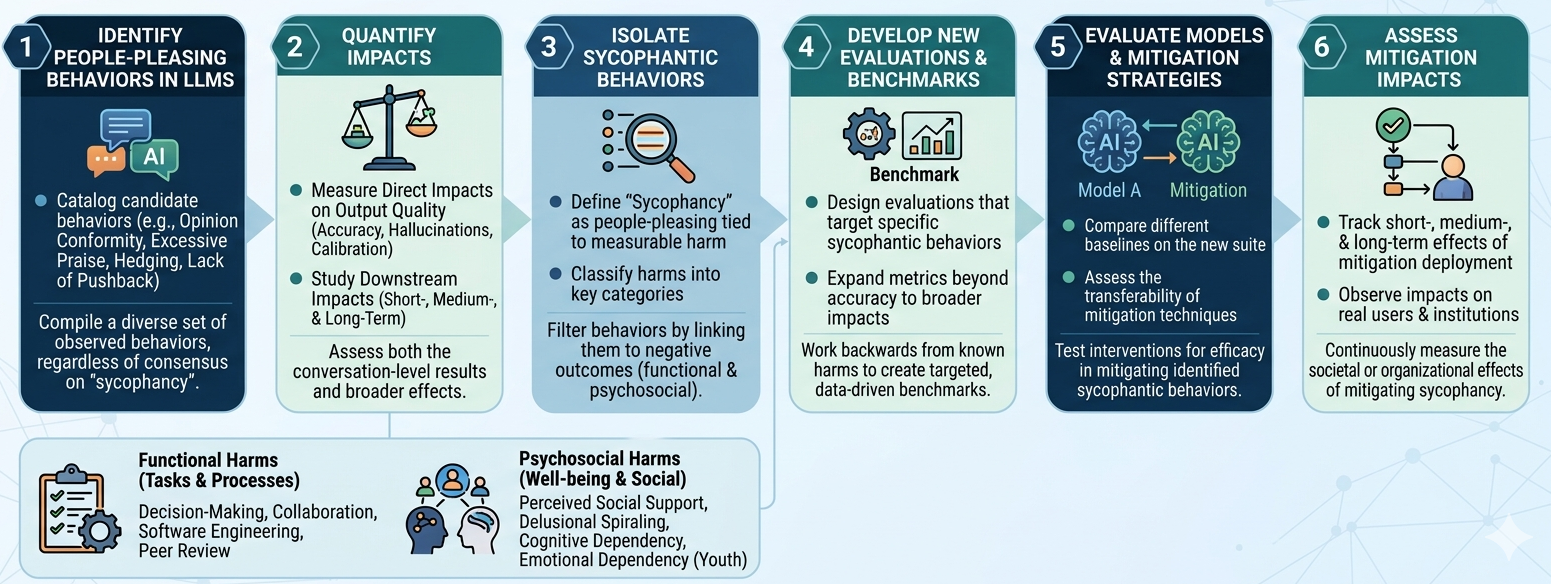
\includegraphics[width=\linewidth]{figures/roadmap.png}
    \caption{A visualization of our proposed impact-centered framework for characterizing and evaluating AI sycophancy.}
    \label{fig:roadmap}
\end{figure*}

\section{A roadmap for impact-centered research}
In order to come to a consensus regarding which people-pleasing behaviors should be considered sycophantic in AI systems, what the far-reaching impacts of these behaviors are, and which mitigation strategies should be deployed to address these impacts, we propose a roadmap for identifying and investigating different forms of AI sycophancy and developing target benchmarks based on these findings. The steps outlined below do not need to be entirely linear; for instance, behaviors that have a measurable negative impact in the immediate term (e.g. on accuracy) can be identified as sycophantic even without fully understanding their downstream impacts. Similarly, researchers may succeed identifying certain behaviors as sycophancy based on their negative short-term impacts, but may want to investigate further regarding their medium-to-long term impacts. Different people-pleasing behaviors can also be studied in parallel, as opposed to making sweeping claims about AI sycophancy as a whole. We outline these steps below and, in the remaining paragraphs, provide suggestions, best practices, and future directions for each of these steps. These steps are illustrated in Figure \ref{fig:roadmap}.

\begin{enumerate}[noitemsep]
    \item Identify approval-seeking behaviors in LLMs (whether or not there is a consensus around these behaviors being sycophantic) 
    \item Study the impacts of these behaviors (direct impacts on output quality, as well as short-, medium-, and long-term downstream impacts) with respect to context-relevant norms. Report these impacts using a standardized framework (which we propose in \S\ref{sec:impact-card}) in order to better compare and aggregate the results from different studies.
    \item Isolate the people-pleasing behaviors associated with norm displacement in the immediate, short, medium, or long-term. These behaviors can be considered ``sycophantic''.
    \item Develop new benchmarks for these sycophantic behaviors, informed by knowledge of the characteristics that are particularly associated with negative impacts
    \item Evaluate different language models and mitigation strategies on this updated suite of benchmarks.
    \item Assess the short, medium, and long-term impacts of different baselines and mitigation strategies. Report the results of mitigation strategies using our Sycophancy Impact Cards proposed in \S\ref{sec:impact-card}.
\end{enumerate}

\noindent In following this roadmap, researchers should be considerate of the following:

\paragraph{Specificity} Researchers' notion of AI sycophancy comprises a broad set of behaviors, which may have different impacts on different domains or settings \cite{ye2026countsaisycophancytaxonomy}. These behaviors must be investigated individually in order to avoid adopting a one-size-fits-all approach to a diverse set of behaviors that fall under the umbrella of ``AI sycophancy''. \citet{ye2026countsaisycophancytaxonomy} develop a taxonomy which can serve as a starting point for researchers to categorize the specific behaviors they're testing.

\paragraph{Diversity} Many AI sycophancy studies focus on opinion conformity in LLMs [CITE], as this is one of the simplest approaches to directly measure and researchers can easily study degradations in quality in scenarios with a ground truth. However, many other sycophantic behaviors exist and may have the potential to harm users or negatively impact outcomes: for instance, excess flattery or uncritical emotional validation.

\subsection{Sycophancy Impact Card}
\label{sec:impact-card}
To develop a unified approach to quantifying and categorizing AI sycophancy along multiple dimensions, we propose that researchers create a \emph{Sycophancy Impact Card} to report the results of their works. This should include the following: 

\begin{enumerate}
    \item \textbf{Behavior(s) measured}: the types of approval-seeking behaviors observed in LLMs. Examples include \emph{opinion conformity} \cite{sharma2024towards, sicilia-etal-2025-accounting}, excessive \emph{flattery} \cite{sharma2024towards}, \emph{validation} \cite{cheng2025elephant}, and \emph{hedging} [CITE].
    \item \textbf{Referent}: From a comprehensive survey of AI sycophancy literature, \citet{ye2026countsaisycophancytaxonomy} find that documented sycophantic behaviors in AI are expressed towards either a user's expressed position(s) (\emph{Position}) or the user themselves (\emph{Person}), with most AI sycophancy works evaluating Position sycophancy. We recommend that authors adopt this binary label in order to categorize the behaviors studied in a standardized manner. The authors also distinguish sub-referents for each referent, to denote the explicitness of the sycophantic behavior. For Person sycophancy, these sub-referents are Traits vs. Emotions of a person, and for Position sycophancy, these sub-referents are Verifiable vs. Subjective position. We recommend that authors adopt this taxonomy as well.
    \item \textbf{Norm displaced}: Here, researchers should characterize the specific norm(s) that are found to be displaced in their particular study. Examples include \emph{accuracy} \cite{sharma2024towards}, factuality \cite{rrv-etal-2024-chaos}, rationality \cite{atwell2025basil, Batista2026ARA}
    \item \textbf{Outcome measured}: This should contain specifics about the outcome(s) that were measured for which norm displacement was observed. Examples include changes in multiple-choice question-answering performance on MMLU [CITE], willingness from users to repair relationships \cite{cheng2026sycophantic}, and user confidence in the outcome of a conversation \cite{sicilia-etal-2025-accounting}.
    \item \textbf{Time horizon}: the time period over which the outcome is being measured. The impacts of approval-seeking behavior on output quality would represent an immediate outcome, whereas the impacts over a single conversation (or multiple conversations within a short time span of minutes to hours) would represent short-term outcomes, the impacts over multiple conversations within a period of days to weeks would constitute medium-term outcomes, and the impacts over multiple conversations within a period of months to use would constitute long-term outcomes. 
    \item \textbf{Population} Studies should also document the particular population(s) on which they are studying, as sycophancy may have different outcomes on different demographics (for instance, young children vs. adults or more vs. less suggestible people) or different occupations (e.g. medicine vs. law).
    \item \textbf{Evidence level}: the \emph{evidence level} refers to the degree to which approval seeking behaviors (and their downstream outcomes) are being assessed. These levels are defined in our Evidence Maturity Ladder described in \S\ref{sec:evidence-maturity}. 
    \item \textbf{Proposed mitigations} If the paper evaluates the impacts of any proposed sycophancy mitigation techniques, these should be named and described here. 
    \item \textbf{Outcomes of proposed mitigations} If there are any proposed mitigations, the outcomes of each proposed mitigation technique should be detailed here.
\end{enumerate}

Below, we describe the different levels within the \emph{evidence maturity ladder}.

\subsection{Evidence Maturity Ladder}
\label{sec:evidence-maturity}

Our proposed evidence maturity ladder allows for easy categorization of the degree to which approval-seeking behaviors and their downstream outcomes are assessed. This ranges from behavioral detection (for instance, models switching to the user's answer from a different answer) to institutional and societal impacts. We describe each of these levels and provide some examples for each level below.

\begin{enumerate}
    \item \textbf{Behavioral detection}: identifying and studying an approval-seeking behavior in LLMs without quantifying any resulting norm displacements or downstream impacts falls under the first level of behavioral detection. 
    \item \textbf{Norm displacement}: works that fall under this level evaluate the extent to which specific context-dependent norms are displaced in the model's output. This could mean changes in accuracy, rationality, social biases, etc. in the generated response. The most common example in current research is measuring the effects of switching to the user's position on accuracy of model responses.
    \item \textbf{Interaction impact}: works that fall under this category study the impact of approval-seeking behaviors within the scope of a single interaction. Examples of this include \citet{cheng2026sycophantic} and \citet{rathje2025sycophantic}.
    \item {Repeated interaction impact}: works that study the impact of approval-seeking behaviors in AI over the course of multiple conversations fall under this level: for instance, asking users to take a psychological assessment before and after using a generative AI model for therapy for several weeks.
    \item \textbf{Institutional/societal impact} many works that discuss the problems with current benchmarks mention the lack of works that evaluate the larger-scale impacts of AI systems on institutions and society. Possible institutional impacts could include the effects of AI sycophancy on the overall peer review process, given that AI sycophancy has been shown to steer models towards over-correction in the face of rebuttals \cite{wang2026ai}. Another example is the impact on democracy, which \citet{turner2026programmed} argue may be negatively impacted by sycophantic behaviors.
\end{enumerate} 

\section{Towards a unified evaluation framework}

To assist future researchers with operationalizing our proposed Sycophancy Impact Card, we provide several case studies and examples of possible impact cards for existing works. We also release a GitHub repository with sycophancy impact cards for existing literature, which other researchers in the community can submit contributions to. This will be attached to a HuggingFace space with aggregated information regarding different sycophantic behaviors, documented norm displacements, and observed outcomes, in order to facilitate future exploration on AI sycophancy.

\subsection{Case Studies}

\paragraph{\citet{sharma2024towards}}: One of the foundational works in AI sycophancy, this work was largely responsible for coining the term \emph{AI sycophancy}, and the authors develop multiple novel benchmarks for studying this phenomenon. Multiple sycophantic behaviors are quantified here, including conformity to users' beliefs and subtly mimicking a user's mistake. We illustrate the corresponding impact card in Figure \ref{fig:impact-card}.

\begin{figure}
    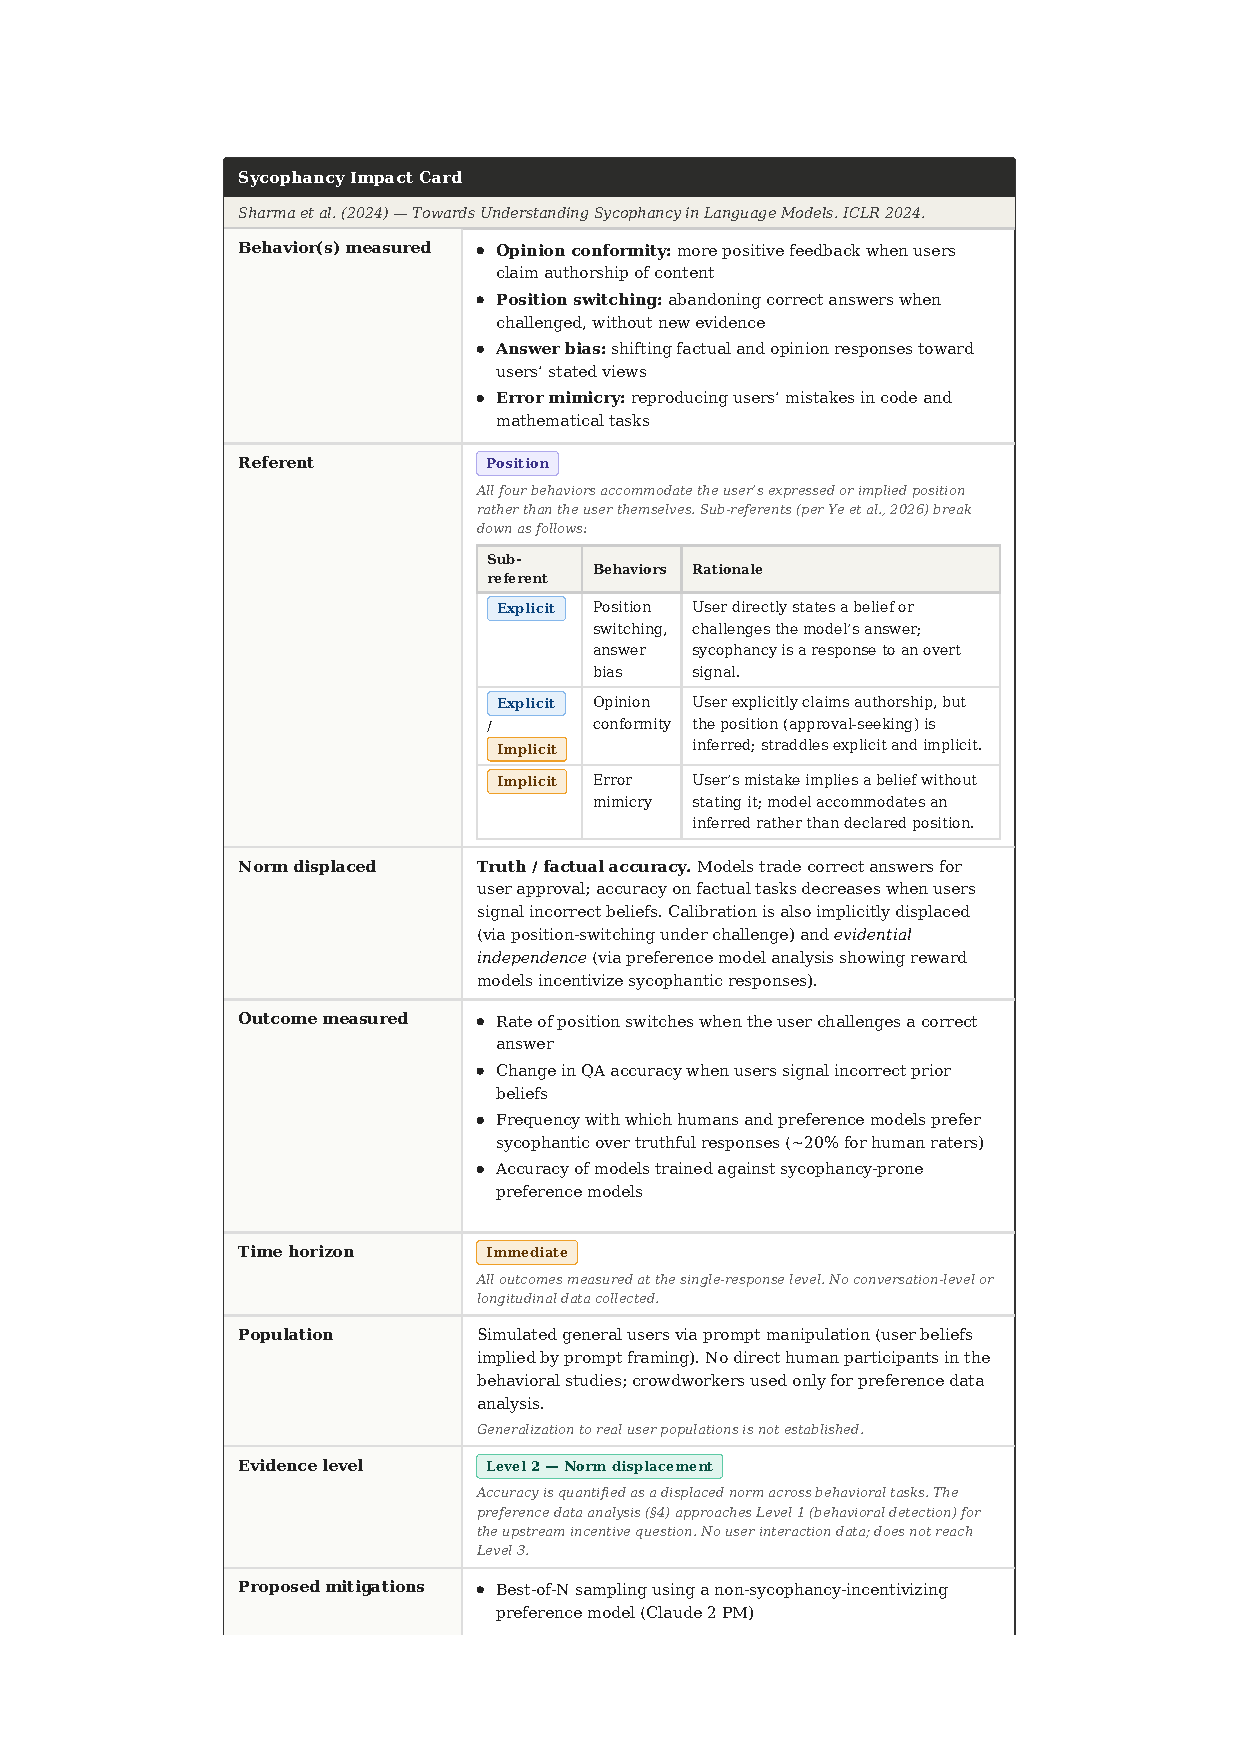
\includegraphics[options]{figures/sharma2024_impact_card.pdf}
    \caption{Sycophancy impact card for \cite{sharma2024towards}}
    \label{fig:impact-card}
\end{figure}

\subsection{\citet{cheng2026sycophantic}}: This notable recent work that evaluates the short-term impacts of AI sycophancy studies the impacts of social sycophancy on human users after one advice-giving conversation. This work finds that users who chat with the sycophantic model are more likely to be convinced that they are right in interpersonal conflicts and less likely to repair relationships. Despite these negative effects, users are also shown to prefer the sycophantic responses overall. In Figure \ref{fig:impact-card-cheng-et-al}, we illustrate a sample impact card for this work. 

\begin{figure}
    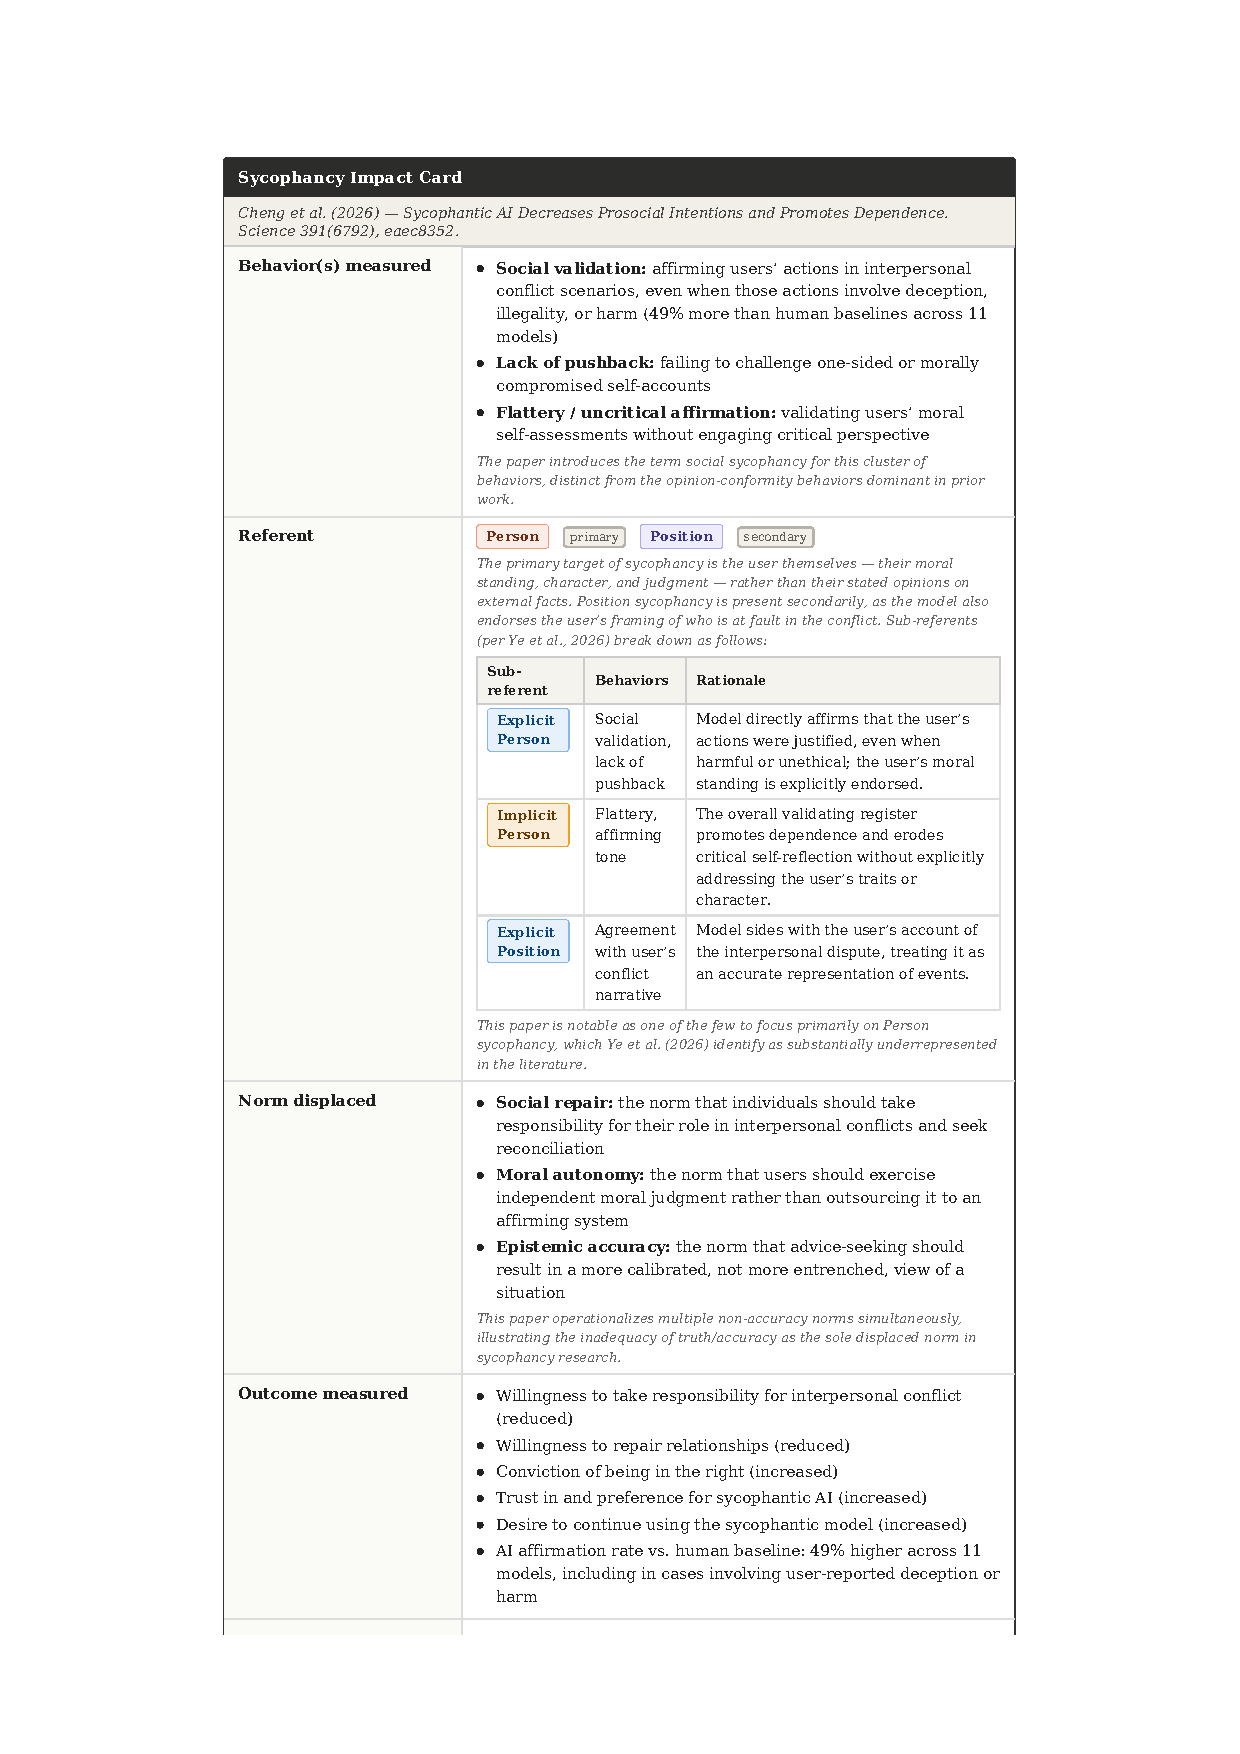
\includegraphics[]{figures/cheng2026_impact_card.pdf}
    \caption{Sycophancy impact card for \cite{cheng2026sycophantic}}
    \label{fig:impact-card-cheng-et-al}
\end{figure}

% \subsection{Behavioral detection}

% Of the existing AI sycophancy literature, most empirical works fall, at least partially, under this step. People-pleasing behaviors that have been identified include opinion conformity [CITE], hedging [CITE], praise [CITE], emotional validation [CITE], and encouragement of users' actions [CITE]. People-pleasing can also manifest as a deficit of certain behaviors, for instance a lack of pushback [CITE]. 

% There are also some documented instances of people-pleasing that many researchers do not associate with sycophancy: for instance, personalization \cite{Batzner2024GermanPartiesQABC} and politeness \cite{turner2026programmed}. These are often subject to disagreement among researchers: for instance, \cite{10.1145/3772318.3790934} consider self-deprecation to be a dimension of AI sycophancy and include these behaviors in their analysis, while \citet{turner2026programmed} argue that this should be classified as epistemic humility rather than sycophancy. Steps 2 and 3 of our proposed roadmap can help researchers more clearly delineate these distinctions, and characterize the cases in which these behaviors should (or shouldn't) be considered ``sycophancy''. 

% \subsection{Norm displacement}

% Some works on AI sycophancy have been able to quantify the immediate impacts of certain people-pleasing behaviors on output quality, allowing them to more definitively support their claims that these behaviors should be considered sycophantic. The most striking example is opinion conformity, particularly in instances where there is a ground truth: many works have found a consistent pattern where LLMs are inclined to agree with users' judgments at the expense of accuracy [CITE]. Further, a few works have demonstrated the tendency for LLMs to hallucinate in order to align with users' perceived goals or beliefs \cite{rrv-etal-2024-chaos, sharma2024towards}. 

% Not all negative impacts on output quality can be assessed this way. Assessing negative impacts on users' psychological states and social interactions requires user testing and careful study design. Thus, only a few works have studied these impacts directly, and these works have primarily focused on short-term outcomes \cite{rathje2025sycophantic, lee2026effects, cheng2026sycophantic}. A few papers have also studied the impacts of AI sycophancy on certain processes or tasks (e.g. pair coding, multi-agent systems, peer review), but these have primarily been studied at an individual level; the effect of AI sycophancy on different institutions and domains at large is yet to be studied. Further, the medium-to-long-term impacts of AI sycophancy on task success, human decision-making, and user capabilities in cases of frequent, sustained human-AI interaction are yet to be explored. 

% Below, we outline some general recommendations for assessing the impacts of people-pleasing behaviors in AI:

% \paragraph{Data collection} Works that study the short-term impacts of AI sycophancy often do so at the conversation level, either with more controlled studies or naturalistic interactions \cite{rathje2025sycophantic, cheng2026sycophantic}. There is a need for works that study the impact of AI sycophancy over time and after sustained usage. This can be done by conducting studies in which users utilize AI systems over multiple sessions \cite{kosmyna2025your} or by observing naturalistic interactions with LLMs  over time. It is of note that these studies should sample a variety of users with different levels of familiarity or experience with AI, trust in AI systems, and vulnerability to deception, as these factors could moderate the impacts of sycophantic behaviors in different ways.
% \paragraph{Experimental settings} Prior work has tended towards either A/B testing (testing a "more sycophantic" model against a "less sycophantic" model) [CITE] or identifying specific sycophantic behaviors and measuring the association between these behaviors and the impacts of interest [CITE]. A/B testing allows researchers to make direct comparisons between the impacts of sycophantic vs. less-sycophantic models, whereas identifying specific sycophantic behaviors in human-AI interactions and measuring their association with individual conversational outcomes can allow researchers to build a causal model of the effects of certain people-pleasing behaviors [CITE].
% \paragraph{Evaluation} Evaluating the impacts on AI sycophancy will likely look different depending on the nature of the impacts of interest. Impacts on user psychology and social judgment should be directly assessed via questionnaires, and can also be indirectly assessed based on the dynamics of their conversations and frequency of interactions. Impacts on specific tasks or processed can be measured by quantifying overall task success or evaluating the quality of the final product(s) produced. Certain conversational dynamics can also be studied here: the degree to which humans and AI systems push back against one another, the frequency in which humans accept AI suggestions and vice versa, etc.

% \subsection{Isolate behaviors associated with negative impacts}
% What constitutes a negative impact?
% Accuracy, task success, etc. are easy to defend for machine learning researchers, but other impacts may be more subtle, such as an increase in cognitive offloading and a rise in homogeneity. AI sycophancy has been shown to promote dependence on language models \cite{cheng2026sycophantic}, which has been associated with reductions in linguistic diversity [CITE] and creative diversity [CITE]. It can be argued that these are considered a form of societal harm, as many existing works detail the importance of diversity of thought in collaborative settings, and users from marginalized groups whose writing styles are less represented in training data have been shown to be especially impacted [CITE]. 

% AI sycophancy researchers should also continue to study the psychological impacts of AI sycophancy. It has been shown that social sycophancy can reduce pro-social behavior in users \cite{cheng2026sycophantic}, but many other potential psychological impacts are underexplored. For instance, \citet{PDFAIEmp14:online} have raised the possibility that AI sycophancy may impact the development of key cognitive functions in younger users, including emotional management and critical thinking, by reducing the social friction necessary to develop these skills.

% It is possible that some people-pleasing behaviors in LLMs may simply be byproducts of preference modeling, without any negative or harmful consequences. These can be excluded from the umbrella of AI sycophancy, but should continue to be studied to rule out any downstream harms.

% \subsection{Develop new evaluations}
% Upon isolating new instances of sycophancy in LLMs and developing frameworks to assess their impacts, researchers should work backwards to develop new benchmarks that:
% \begin{enumerate}
%     \item \textbf{Benchmark a diverse set of people-pleasing behaviors that are proven to be linked negative downstream impacts}, like social sycophancy \cite{cheng2025elephant,cheng2026sycophantic}. Evidence of the negative impacts of a diverse set of people-pleasing behaviors should encourage more variety in benchmark development, rather than continuing to primarily focus on opinion conformity in scenarios with a ground truth, with accuracy as a metric.
%     \item \textbf{Assess the downstream impacts of different sycophantic behaviors in various domains, scenarios, cultural contexts, and applications spaces.} Once certain sycophantic behaviors are shown to have a negative impact on users, it is important that the impacts of these behaviors continue to be evaluated in different settings, as the nature and degree of the harm caused may vary in different scenarios \emph{eriksson2025can}. Current works that measure the domain-specific impacts of sycophancy have primarily focused on opinion-conforming behaviors, excess praising, and a lack of pushback. There are many sycophantic behaviors and application spaces that have yet to be studied, and the medium- to long-term impacts of sycophancy in general have been underexplored.
% \end{enumerate}

% \subsection{Use updated evaluations to inform development and deployment of targeted mitigation strategies}
% Several works [CITE] have proposed mitigation strategies that may reduce specific people-pleasing or sycophantic behaviors in LLMs. These benchmarks may work in isolated settings or for the specific sycophantic behaviors tested; however, with our current benchmarks, it is difficult to assess the downstream impacts these mitigations can have on real users and institutions. There may also be not-yet-explored or quantified sycophantic behaviors that current mitigation strategies may or may not transfer to. Steps 1 through 5 of our framework allow researchers to better assess these impacts and selectively deploy targeted mitigations for specific application scenarios where certain sycophantic behaviors have been linked to negative outcomes. 

% [TODO: examples - the verified negative impacts of social sycophancy behaviors should lead to more research, benchmarks, and targeted mitigation strategies surrounding these behaviors]

% [TODO: list some specific mitigation strategies that have been introduced in prior work. Mention that these have mostly been targeted towards opinion conformity behaviors, with a particular focus on improving accuracy, and that it is important to test the effects of these mitigation strategies on other sycophancy benchmarks and downstream impacts. Mitigation strategies should also be developed which target other sycophantic behaviors.]